\documentclass[a4paper,12pt]{amsart}

\usetheme[progressbar=frametitle]{metropolis}
\metroset{block=fill}

\subtitle{NTIN071 Automata and Grammars}
\author{Jakub Bulín (KTIML MFF UK)}

\date{Spring 2025\\ 
    \vspace{1in} 
    \begin{flushleft}
        \it \footnotesize * Adapted from the Czech-lecture slides by Marta Vomlelová with gratitude. The translation, some modifications, and all errors are mine.
    \end{flushleft}
}

%% packages

\usepackage{amsmath}
\usepackage{amssymb}
\usepackage{amsthm}
\usepackage{cancel}
\usepackage{color}
\usepackage{colortbl}
\usepackage{forest}
\usepackage[utf8x]{inputenc}
\usepackage{multicol}
\usepackage{multirow}

%% colors
\definecolor{Gray}{gray}{0.9}

%% TikZ
\usepackage{tikz}
    \usetikzlibrary{
        automata,
        arrows,
        backgrounds,
        decorations.pathmorphing,
        fit,
        positioning,
        shapes,
        shapes.geometric,
        tikzmark
    } 
    \tikzset{>=stealth',shorten >=1pt,auto,node distance=2cm}
    \tikzset{initial text={}}
    \tikzset{elliptic state/.style={draw,ellipse}}

%% amsthm
\theoremstyle{plain}
    \newtheorem*{algorithm}{Algorithm}    
    \newtheorem*{observation}{Observation}
    \newtheorem*{proposition}{Proposition}

\theoremstyle{remark}
    \newtheorem*{exercise}{Exercise}
    \newtheorem*{remark}{Remark}

%% macros
\DeclareMathOperator{\RegE}{RegE}
\DeclareMathOperator{\RL}{RL}

% Just for Lecture 2
\newcommand{\x}{$\times$}
\newcommand{\nx}{\ }


\begin{document}

\thispagestyle{empty}

\section*{NTIN071 A\&G: Cvičení 6 -- Formální gramatiky, regulární a bezkontextové gramatiky}

\medskip

\subsection*{Cíle výuky:} Po absolvování student umí

\begin{itemize}\setlength{\itemsep}{0pt}
    \item vysvětlit formální definici gramatiky a jazyka, který generuje,
    \item uvést definice a příklady gramatik všech typů v Chomského hierarchii,
    \item popsat jazyk generovaný danou bezkontextovou gramatikou,
    \item sestrojit gramatiku pro jazyk zadaný v množinové notaci,
    \item převést konečný automat na pravou lineární gramatiku,
    \item převést pravou lineární gramatiku na konečný automat,
    \item navrhnout algoritmy pro testování základních vlastností bezkontextových gramatik.
\end{itemize}


\section*{Příklady na cvičení}


\medskip\begin{problem}[Konstrukce gramatik]

    Navrhněte gramatiky (co nejvyššího typu), které generují následující jazyky ($\Sigma=\{a,b\}$, není-li řečeno jinak):
    
    \vspace{-3pt}
    \begin{multicols}{2}
    \begin{enumerate}[(a)]
        \item $L=\{w\in\Sigma^*\mid |w|_b\text{ je sudý}\} $
        \item $L=\{ww^R\mid w\in \Sigma^*\}$        
        \item $L = \{a^ib^jc^k\mid i = j\text{ nebo }j = k\}$        
        \item $L=\{a^i b^j\mid 0\leq i\leq j\leq 2i\}$
        \item $L=\{uabbav\mid u,v\in\Sigma^*\text{ a }|u|=|v|\}$
        \item $L=\{w\in \Sigma^*\mid -1\leq |w|_a-|w|_b\leq 1\}$        
    \end{enumerate}
    \end{multicols}

\end{problem}


\begin{problem}[Z konečného automatu na gramatiku]

    Pro následující konečný automat nalezněte ekvivalentní gramatiku. V jaké třídě Chomského hierarchie se budete pohybovat?
    
    \vspace{-6pt}
    \begin{center}
        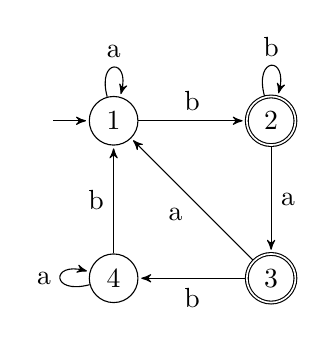
\begin{tikzpicture}[>=stealth',shorten >=1pt,auto,node distance=2cm]
            \tikzset{every state/.style={minimum size=0.2cm}}			
            \node[initial,state]  (a1)      {1};
            \node[state,accepting] (b1)  [right of=a1]    {2};
            \node[state,accepting] [below of=b1](c1)      {3};
            \node[state] [below of=a1](d1)      {4};
            \path[->]
                (a1)  edge  node {b} (b1)
                (a1)  edge[loop above]  node {a} (a1)
                (b1)  edge[loop above]  node {b} (b1)
                (d1)  edge[loop left]  node {a} (d1)
                (b1)  edge  node {a} (c1)
                (c1)  edge  node {a} (a1)
                (c1)  edge  node {b} (d1)
                (d1)  edge  node {b} (a1);
        \end{tikzpicture}
    \end{center}
        
\end{problem}


\begin{problem}[Z regulární gramatiky na konečný automat]
    
    Převeďte následující pravou lineární gramatiku na konečný automat: $G=(\{S,A,B,C\},\{a,b\},\mathcal P,S)$, kde $\mathcal P$ sestává z:

    \medskip
        
    \begin{center}
        \begin{tabular}{l}
            $S\rightarrow abS\mid babA\mid \epsilon $\\
            $A\rightarrow abA\mid aB \mid  bC$\\
            $B\rightarrow abS\mid B\mid bC\mid \epsilon $\\
            $C\rightarrow aab\mid A\mid aA\mid \epsilon $
        \end{tabular}
    \end{center}
    
\end{problem}


\begin{problem}[Testování vlastností bezkontextových jazyků]

    Vymyslete (co nejefektivnější) algoritmus, který rozhodne, zda daná bezkontextová gramatika splňuje danou vlastnost:
    
    \vspace{-6pt}
    \begin{multicols}{3}
    \begin{enumerate}[(a)]
        \item $L(G)\neq\emptyset$
        \item $\epsilon\in L(G)$
        \item $L(G)$ je konečný jazyk
    \end{enumerate}
    \end{multicols}

\end{problem}


\section*{K procvičení a k zamyšlení}


\medskip\begin{problem}[Konstrukce gramatik]

    Navrhněte gramatiky (co nejvyššího typu), které generují následující jazyky ($\Sigma=\{a,b\}$, není-li řečeno jinak):
    
    \begin{enumerate}[(a)]    
        \item $L=\Sigma^*$        
        \item $L=\{a^{2i}b^j\mid i\leq j\}$
        \item $L=\{w\in\Sigma^*\mid |w|_a = 2|w|_b\}$        
        \item $L=\{uabbav\mid u,v\in\Sigma^*\text{ a platí }|u|\neq|v|\}$ 
        \item $L = \{w \# s^R \mid w,s\in\Sigma^*\text{ a $s$ je podslovo slova $w$}\}$
    \end{enumerate}

\end{problem}


\medskip\begin{problem}[Malé gramatiky generující velké (konečné) jazyky]
    
    Najděte posloupnost bezkontextových gramatik $G_1,G_2,G_3,\dots$ (nad danou abecedou $\Sigma$) takových, že $G_n$ generuje právě všechna slova délky $\leq 2^n$ (a žádná jiná), a přitom velikost $G_n$ (pro jednoduchost počet symbolů v tělech produkčních pravidel) je v $O(n)$.
    
    %X_1 \to X_2_X2, X_2 \to X_3X_3,\dots, X_{n−1}\to X_nX_n, X_n\to aa|a|\epsilon

\end{problem}


\end{document}
